\documentclass{worksheet}

\solutiontrue
% \solutionfalse

\assignmenttitle{Lecture 90 Worksheet}
\assignmentcourse{\textsc{Subject 1234: Course title}}
\assignmentsemester{Summer 2099}
\assignmentduedate{Apr 34}
\instructorname{Firstname Lastname}
\lecturetitle{Lecture Topic}
\lecturesummary{A brief summary of lecture.}


\begin{document}
    \thispagestyle{empty}
	\maketitle
    \vspace{-1em}
	
 
	\section{First Section}
    
    Uses kpfonts.
	
	\begin{defn}[Definition Title]{label_defn1}
	A definition. The title is optional.
	\end{defn}
	    
	We can have numbered list as follows:
    \begin{enumerate}
    
    \item  Vectors and Matrices are written as $\vec{r}(t)=\begin{bmatrix}1 & 2\\ 3 & 4\end{bmatrix}$.
    
    \item Typewriter font is written as {\tt Computer Code}.
    \end{enumerate}
    
    or itemized list as follows:
    
    \begin{itemize} %Use the itemize environment to make an unordered list.
    
    
            
    \item Here is how to write a table such as \cref{table:arrows}.
    
     
    \begin{table}[!ht]
            \renewcommand{\arraystretch}{1.5} %Use this multiplier to increase row height
            \centering
            \begin{tabular}{c|c|c|c|}
            {} & $f(x,y)<0$ & $f(x,y)=0$ & $f(x,y)>0$  \\
            \hline
            $g(x,y)<0$ & $\swarrow$ & $\downarrow$ & $\searrow$ \\
            \hline
            $g(x,y)=0$ & $\leftarrow$ & $\cdot$ & $\rightarrow$ \\
            \hline
            $g(x,y)>0$ & $\nwarrow$ & $\uparrow$ & $\nearrow$ \\
            \hline
            \end{tabular}
            \caption{Arrows}
            \label{table:arrows}
    \end{table}
    
    \item  When we need more than one line to align nicely:
           	\begin{align*}
        	    y' &= \mu - y^2 &\text{\em (saddle-node)}\\ %Emphasis is orange and bold by default
        	    y' &= \mu y - y^2 &\text{\em (transcritical)}\\
        	    y' &= \mu y -y^3 &\text{\em (supercritical pitchfork)}\\
        	    y' &= \mu y +y^3 &\text{\em (subcritical pitchfork)}
        	\end{align*}

    
    \item If you need to label each line, you can get rid of the star from {\tt align*}
            \begin{align}
                \frac{dx}{dt} &= f(x,y,t) \\ 
        	    \frac{dy}{dt} &= g(x,y,t)
            \end{align}
    
    \item 
    You can insert figures such as \cref{fig:arcsin} as follows:
    \begin{figure}[!ht] % This means draw the figure either [h]ere, as in right after previous line, or at the [t]op of the page if there's not enough space
        \centering
        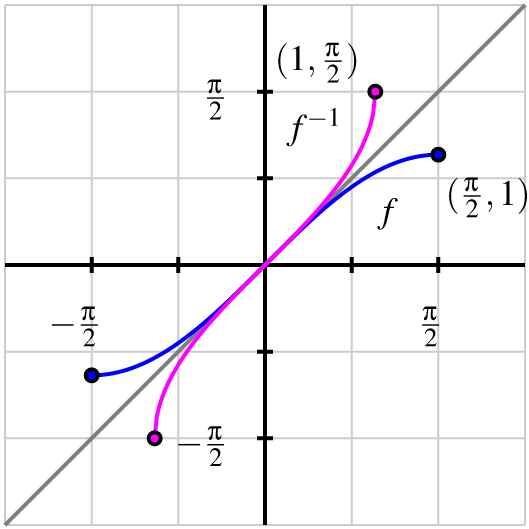
\includegraphics[width=0.4\textwidth]{images/picture.png}
        \caption{$\arcsin x$}
        \label{fig:arcsin}
    \end{figure}
    
    \end{itemize}
   
	
	
	
	\begin{exmpl}[Title]{label_exmpl}
	 \begin{itemize}
        \item First example 
        \begin{itemize}
            \item  Note $1$
            \item  Note $2$
        \end{itemize}
        \item Second example
    \end{itemize}
	\end{exmpl}    


    
	Some other text.
	
	\begin{theo}[Theorem Title]{label_thm}
	A Theorem that uses objects defined in \cref{label_defn1}. Title is optional. 
	\[\dint_a^b u v' \dx = [u(x)v(x)] \eval_a^b - \dint_a^b u'(x) v(x) \dx\]
	\end{theo}
	
    
    \begin{prf}{label_thm}
    Proof text ends in qed symbol. Must be supplied the label of the theorem.
    \end{prf}
    

    \paragraph{Automatic Question numbers in References}
    \begin{enumerate}
        \item Greek letters and uppercase math letters are always upright. Such as \label{step_a}
        \begin{enumerate}
            \item  $\alpha x^2 +\beta$ \label{substep_a_i} 
            \item  $y =mx+ C \in \R$ 
        \end{enumerate}
   
        \item Do the  following tasks after \ref{step_a}.
        \begin{tasks}(3)
        \task first do \ref{substep_a_i}.
        \task ??    
        \task Profit
        \end{tasks}
    \end{enumerate}
    
    % \eoq %This is usually not needed, only used for formatting nicely.
    
    \begin{solution}
    Solution to the exercise. Uncomment the ``solutionfalse'' flag to make solutions invisible.
    \end{solution}
    
    
    \begin{note}[Fun Fact:]
	This is a note with a custom title. Default is `Note:'.
	\end{note}
	
	
%%%%%%%%%%%%%%%%%%%%%%
%\newpage %Uncomment to force a page break
%%%%%%%%%%%%%%%%%%%%%%
    
	\section{Second Section}
	
	\begin{axiom}{label_axiom}
	This is an axiom.
	\end{axiom}
	
	
	
    \begin{code}[Code:]
    \begin{verbatim}
    	$ chmod +x hello.py
    	$ ./hello.py
    	
    	Hello World!
    \end{verbatim}
    \end{code}
	
	\begin{digression}
	    A digression into tangentially related topics.
	\end{digression}
    
    
    
    \subsection{Case 1: First case}
    When  \cref{label_exmpl} is true.
    \begin{warning}[A Warning:] %default is Warning:
     \lipsum[1][1-2]
    \end{warning}
    
    \subsection{Case 2: Second case}
    When example \ref{label_exmpl} is false.
        
        \subsubsection{Important Topic}
        \lipsum[2]
	
	\sectionline{orange}{88}
\end{document}	

